\documentclass{beamer}
\usepackage[T1]{fontenc}
\usepackage[utf8]{inputenc}
%\usepackage{dsfont}
\usepackage{lmodern}
\usepackage{amsmath}
\usepackage{amssymb}
\usepackage{graphics}
\usepackage{multimedia}
\usepackage{multicol}
\usepackage[percent]{overpic}
%\usepackage{biblatex}


%%%%%%%%%%%%%%%%%%%%%%%%%%%%%%%%%%%%%%%%%%%%%%%%%%%%%%%%%%%%%%%%
%%%%%%%%%%%%%%%%%%%% Python code %%%%%%%%%%%%%%%%%%%%%%%%%%%%%%%
%%%%%%%%%%%%%%%%%%%%%%%%%%%%%%%%%%%%%%%%%%%%%%%%%%%%%%%%%%%%%%%%

\usepackage{listings}
% the following lines make sure the pdf code is copy-pastable
\usepackage{textcomp}
\usepackage[space=true]{accsupp}

\newcommand{\pdfactualhex}[3]{\newcommand{#1}{%
		\BeginAccSupp{method=hex,ActualText=#2}#3\EndAccSupp{}}}

\pdfactualhex{\pdfactualdspace}{2020}{\textperiodcentered\textperiodcentered}
\pdfactualhex{\pdfactualsquote}{27}{'}
\pdfactualhex{\pdfactualbtick}{60}{`}

% define colours 
\definecolor{deepblue}{rgb}{0,0,0.8}
\definecolor{deepred}{rgb}{1.0,0,0}
\definecolor{deepgreen}{rgb}{0,0.7,0}
\definecolor{blueviolet}{RGB}{138,43,226}
\definecolor{darkyellow}{RGB}{204,204,0}
\definecolor{codegray}{rgb}{0.6,0.6,0.6}
\definecolor{weborange}{RGB}{255,165,0}
\definecolor{gold}{RGB}{255,205,0}
\definecolor{codegreen}{rgb}{0,0.6,0}
\definecolor{codepurple}{rgb}{0.58,0,0.82}

%\definecolor{backcolour}{rgb}{0.0,0.0,0.0}
\definecolor{backcolour}{rgb}{0.95,0.95,0.92}

\lstdefinestyle{sublime}{
	backgroundcolor=\color{backcolour},   
	commentstyle=\color{deepgreen},
	keywordstyle=\color{deepred},
	numberstyle=\tiny,
	stringstyle=\color{weborange},
	basicstyle=\tiny\ttfamily, %\footnotesize,
	breakatwhitespace=false,         
	breaklines=true,                 
	captionpos=t,                    
	keepspaces=true,                 
	numbers=left,                    
	numbersep=5pt,                  
	showspaces=false,                
	showstringspaces=false,
	showtabs=false,                  
	tabsize=4,
	columns=flexible,
	emptylines=10000,
	literate={'}{\pdfactualsquote}1{`}{\pdfactualbtick}1{\ \ }{\pdfactualdspace}2,
	inputpath=./anc,
	keywords={lambda,xrange,abs,for,return},
}
\lstset{style=sublime,language=Python}

% change default listings caption title
\renewcommand{\lstlistingname}{\emph{Code Snippet}}% Listing -> q\spin\ Example Code


%%%%%% the following lines put the slashed zero in the code environtmnet listings

\usepackage{marvosym,etoolbox}
% this replaces 0 with \0 in lstings
\lstset{literate={0}{\0}1{0\ }{\0\ }2}

\renewcommand*\ttdefault{txtt}
\usepackage[T1]{fontenc}
\usepackage{graphicx}
% defines \0 as mirro of 0
\newcommand\0{\scalebox{-1}[1]{0}}
% fix for \texttt and \ttfamily
\let\svttfamily\ttfamily
\let\svtexttt\texttt
\catcode`0=\active
\def0{\0}
\renewcommand\ttfamily{\svttfamily\catcode`0=\active }
\renewcommand\texttt{\bgroup\ttfamily\texttthelp}
\def\texttthelp#1{#1\egroup}
\catcode`0=12 %

%%%%%%%




% Style
\usetheme{Warsaw}
\usefonttheme{serif}
\usecolortheme{beaver}
%\useoutertheme{infolines}

\newcommand{\pz}{\sigma^z}
\newcommand{\px}{\sigma^x}
\newcommand{\py}{\sigma^y}
\newcommand{\id}{\mathbb{I}}
\newcommand{\intro}{QuSpin_intro.py}
\newcommand{\qcp}{QuSpin_qcp.py}



\begin{document}
	
\title[weinbe58@bu.edu]{ED methods with QuSpin}
\author{Phil Weinberg}

\date{\today}


\begin{frame}
	\titlepage
\end{frame}

\begin{frame}
	\frametitle{Exact diagonalization (ED) \\ and Quantum Many-body Systems.}
	Many interesting experimental setups are not in a position to probe many-body systems with non-pertubative couplings in order to understand certain phenomena for example:
	\begin{itemize}
		\item Quantum phase transitions.
		\item Quantum thermalization and Many-body localization. 
		\item strongly out of equilibrium dynamics.
	\end{itemize}
	
	Exact diagonalization methods are limit to small system sizes ($N\sim O(20)$) only by the memory and calculation time requirements.
	
	One tool for these kind of calculations is called QuSpin. An open source python library for doing ED calculations. 

\end{frame}

\begin{frame}
\frametitle{Many-Spin Hilbert Space}
\begin{itemize}
\item Hilbert space for spin-$1/2$ consists of $2^N$ states.
\item  We define kets of spin configurations for $N$ spins with site index increasing from left to right $|\overrightarrow{\uparrow\downarrow\downarrow...}\rangle$.
\end{itemize}
 These spin configs can be mapped to integers using binary numbers:
\begin{gather*}
|\uparrow\downarrow\downarrow...\rangle\rightarrow|100...\rangle\rightarrow|2^N-b_s-1\rangle\\\mathrm{or...}\\
|\uparrow\downarrow\downarrow...\rangle\rightarrow|011...\rangle\rightarrow|b_s\rangle
\end{gather*}
which for $N=2$:
\begin{gather*}
|\uparrow\uparrow\rangle\rightarrow |11\rangle\rightarrow|0\rangle\\
|\uparrow\downarrow\rangle\rightarrow |10\rangle\rightarrow|1\rangle\\
|\downarrow\uparrow\rangle\rightarrow |01\rangle\rightarrow|2\rangle\\
|\downarrow\downarrow\rangle\rightarrow |00\rangle\rightarrow|3\rangle
\end{gather*}
\end{frame}

\begin{frame}
	\frametitle{Two-Spin Example}
	explicitly we can construct some of the operators for two spins. $\sigma^\alpha_i$ are the pauli-matricies for the $i^\mathrm{th}$ spin.
	\begin{columns}
		\begin{column}{0.45\textwidth}
			\begin{gather*}
				\pz_0\pz_1 =
				\begin{bmatrix}
				1 & 0 & 0 & 0 \\
				0 & -1 & 0 & 0 \\
				0 & 0 & -1 & 0 \\
				0 & 0 & 0 & 1
				\end{bmatrix}\\
				\px_0=
				\begin{bmatrix}
				0 & 0 & 1 & 0 \\
				0 & 0 & 0 & 1 \\
				1 & 0 & 0 & 0 \\
				0 & 1 & 0 & 0
				\end{bmatrix}\\
				\px_1=
				\begin{bmatrix}
				0 & 1 & 0 & 0 \\
				1 & 0 & 0 & 0 \\
				0 & 0 & 0 & 1 \\
				0 & 0 & 1 & 0
				\end{bmatrix}
			\end{gather*}
		\end{column}
		\begin{column}{0.45\textwidth}
			H-space:
			\begin{gather*}
				|\uparrow\uparrow\rangle\rightarrow |11\rangle\rightarrow|0\rangle\\
				|\uparrow\downarrow\rangle\rightarrow |10\rangle\rightarrow|1\rangle\\
				|\downarrow\uparrow\rangle\rightarrow |01\rangle\rightarrow|2\rangle\\
				|\downarrow\downarrow\rangle\rightarrow |00\rangle\rightarrow|3\rangle\\
			\end{gather*}
			example calculation:
			\begin{gather*}
				\px_0|0\rangle = \px_0|\uparrow\uparrow\rangle = |\downarrow\uparrow\rangle=|2\rangle\\
				\px_0|1\rangle = \px_0|\uparrow\downarrow\rangle = |\downarrow\downarrow\rangle=|3\rangle\\
				\px_0|2\rangle = \px_0|\downarrow\uparrow\rangle = |\uparrow\uparrow\rangle=|0\rangle\\
				\px_0|3\rangle = \px_0|\downarrow\downarrow\rangle = |\uparrow\downarrow\rangle=|1\rangle
			\end{gather*}

		\end{column}
	\end{columns}
\end{frame}




\begin{frame}
\frametitle{Non-Branching Operators}
Previous example showed only one matrix element per column. This turns out to be general for any product Pauli-matrices e.g.
\begin{equation*}
	\left(\prod_j\sigma^{\alpha_j}_{i_j}\right)|s\rangle= M|s'\rangle
\end{equation*}
individual operators only act on the local H-space:
\begin{align*}
\pz_i|...\uparrow...\rangle= |...\uparrow...\rangle&,\quad \pz_i|...\downarrow...\rangle=-|...\downarrow...\rangle\\
\px_i|...\uparrow...\rangle=|...\downarrow...\rangle&,\quad\px_i|...\downarrow...\rangle=|...\uparrow...\rangle\\
\py_i|...\uparrow...\rangle=i|...\downarrow...\rangle&,\quad\py_i|...\downarrow...\rangle=-i|...\uparrow...\rangle
\end{align*}
These kinds of operators are called \emph{non-branching} operators. Operators also commute in the sense that:
\begin{equation}
\sigma^\alpha_i\sigma^\beta_j|s\rangle = \sigma^\beta_j\sigma^\alpha_i|s\rangle\quad (i\ne j)
\end{equation}
\end{frame}

\begin{frame}
\frametitle{QuSpin, python package for ED}
QuSpin is ED package for python which does lots of different kind of ED calculations:
\begin{itemize}
\item Construct both local and non-local operators with both static and time dependent coefficients for Spin, Boson, and Fermion systems.
\item Calculate Eigenvalues and Eigenvectors of operators.
\item Calculate time evolution under the Schroedinger equation with operators. 
\item Calculate entanglement entropy and partial traces of quantum states. 
\item ... 
\end{itemize}
check out the website: http://weinbe58.github.io/QuSpin/ and you can find an in depth introduction: SciPost Phys. 2, 003 (2017).

\end{frame}
\frametitle{Installation if QuSpin.}

\begin{frame}
Installing python+QuSpin(all operating systems):
\begin{itemize}
\item install Anaconda Python package manager for your OS. 
\item type \texttt{conda install -c weinbe58 QuSpin} into command line and follow prompts. 
\end{itemize}

Notes about python:
\begin{itemize}
\item Python run with an interpreter, to run script from command line type: \texttt{python <name\_of\_script>.py}
\end{itemize}
\end{frame}
\begin{frame}
\frametitle{Using QuSpin 1}
Example: Transverse field ising chain. Hamiltonian is given by:
\begin{equation*}
H(s) = -s\sum_{i=0}^{L-1} \pz_i\pz_{i+1} - (1-s)\sum_{i=0}^{L-1}\px_i
\end{equation*}
with periodic boundary conditions $i=L=0$. Lets go over how to build our hamiltonian for a fixed value of $s$.

\end{frame}

\begin{frame}[t]
\frametitle{Using QuSpin 2}
setting up a script, it is good practice to import all neccesary packages before writing any of your own code:
\lstinputlisting[firstline=1, lastline=3, firstnumber=1]{\intro}
Next we set the parameters of our Hamiltonian:
\lstinputlisting[firstline=5, lastline=7, firstnumber=5]{\intro}
Next we define the Hilbert space which we plan on using by defining a basis object. This object is needed to tell QuSpin what kind of many-body operators to construct.
\lstinputlisting[firstline=8, lastline=10, firstnumber=8]{\intro}
Next we need to tell QuSpin which operators to construct. 

\end{frame}

\begin{frame}[t]
\frametitle{Using QuSpin 3}
\begin{itemize}
\item In QuSpin, operators $J\sigma_{i_1}^{\alpha_1}\cdots\sigma_{i_n}^{\alpha_n}$ are defined by an n-letter string "$\alpha_1...\alpha_n$" representing operator types, $\alpha_i\in\left\lbrace +,-,z,x,y\right\rbrace$ together with a site-coupling list $\left[J,i_1,...,i_n\right]$ which holds the lattice site index $i$ for each spin operator in the string. 
\item For a given operator string we associate with it a list of site-couplings.
\item Operator strings are split between static and dynamic pieces where time dependence is given by a user defined function. 
\end{itemize}
Examples:
\begin{center}
\begin{tabular}{|c|c|c|}
	\hline
	operator &  string & site-coupling list \\
	$-s\sum_{i=0}^{L-1}\pz_i\pz_{i+1}$ & \texttt{"zz"} & \texttt{[[-s,0,1],...,[-s,L-1,0]]} \\
	\hline
	$-(1-s)\sum_{i=0}^{L-1}\px_i$ & \texttt{"x"} & \texttt{[[-(1-s),0],...,[-(1-s),L-1]]} \\
	\hline
\end{tabular}
\end{center}
\end{frame}

\begin{frame}[t]
\frametitle{Using QuSpin 4}
Now in the code we define the site-coupling lists for the ising term and the transverse field, and construct the Hamiltonian object:
\lstinputlisting[firstline=11, lastline=18, firstnumber=11]{\intro}
variable \texttt{H} will now be used to calculate all sorts of things. In this example we show how to diagonalize the matrix using a few different methods:
\lstinputlisting[firstline=19, lastline=25, firstnumber=19]{\intro}

\end{frame}


\begin{frame}
\frametitle{Using QuSpin 5}
Full code: \texttt{QuSpin\_intro.py}
\lstinputlisting[firstline=1, lastline=25, firstnumber=1]{\intro}
\end{frame}

\begin{frame}
\frametitle{Using QuSpin 6}
More complicated code, looping over values of $s$: \texttt{QuSpin\_qcp.py}
\lstinputlisting[firstline=1, lastline=32, firstnumber=1]{\qcp}
\end{frame}

\begin{frame}
\frametitle{Using QuSpin 7}
Using lattice symmetries like translational invariance or parity, the system sizes one can calculate increases. In QuSpin one can take advantage of these symmetries by simply specifying them when constructing the basis object:

\texttt{basis=spin\_basis\_1d(L,S="1/2",Pauli=True,kblock=...)}
\begin{figure}
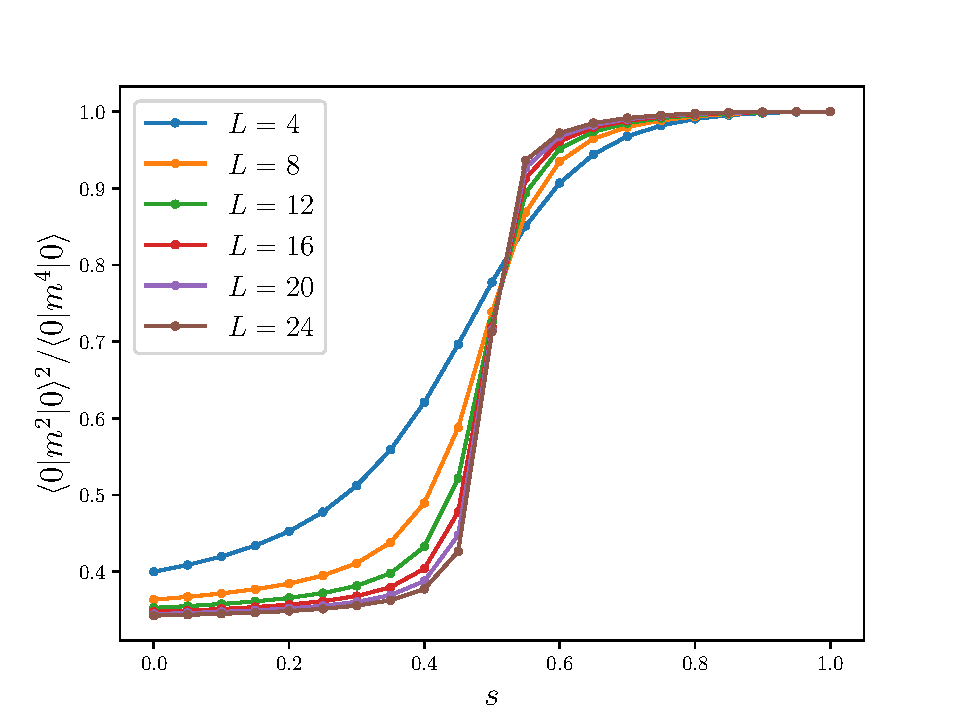
\includegraphics[width=0.6\textwidth]{anc/B.pdf}
\end{figure}
Bonus example, time evolution: \texttt{QuSpin\_anneal.py}
\end{frame}



\begin{frame}
	\frametitle{Using QuSpin 8}
	Using bi-conjugate gradient to solve for spectral functions:
	\begin{equation*}
		S(\omega) = -\frac{1}{\pi}\langle 0 |A^\dagger \frac{1}{\omega+i\eta+E_0-H} A|0\rangle
	\end{equation*}
	define: $|A\rangle = A|0\rangle$, solve
	\begin{equation}
		(\omega+i\eta+E_0-H)|x(\omega)\rangle = |A\rangle
	\end{equation}
	then,
	\begin{equation}
		S(\omega) = -\frac{1}{\pi}\langle A|x(\omega)\rangle
	\end{equation}
	Bonus example: \texttt{QuSpin\_spectral\_function.py}
	
	
\end{frame}




\end{document}
